\documentclass[11pt,aps,preprint,nofootinbib,superscriptaddress,tightenlines]{revtex4-2}
\usepackage[T1]{fontenc}
\usepackage{amsmath,amssymb,mathtools,bm}
\usepackage{xcolor}
\usepackage{booktabs}
\usepackage{graphicx}
\usepackage{dsfont}
\newcommand{\one}{\mathds{1}}
\newcommand{\avg}[1]{\langle #1\rangle}
\newcommand{\klab}{\mathcal B}
\definecolor{darkblue}{RGB}{20,60,140}
\usepackage[colorlinks=true,linkcolor=darkblue,citecolor=darkblue,urlcolor=darkblue]{hyperref}

\def\st{\begin{equation}}
\def\stp{\end{equation}}
\def\Eq#1{eq.~(\ref{#1})}
\def\Sect#1{Sect.~\ref{#1}}
\def\Fig#1{Fig.~\ref{#1}}
\let\oldparagraph\paragraph
\renewcommand{\paragraph}{\par\bigskip\oldparagraph}

\begin{document}
\sloppy

\title{Renormalization of the particle Hamiltonian: a review}
\author{D.~Teaney}
\affiliation{Department of Physics and Astronomy, Stony Brook University,
Stony Brook, New York 11794, USA}
\date{\today}

\begin{abstract}
A particle of the stochastic SPH model carries an entropy $s_a$, a momentum and a volume.  With the energy of the target fluid as its Hamiltonian
(the tree level), the canonical ensemble of the particles has the target equation of state only up to terms of relative order $1/s_a$: the ideal
gas of the labels and the Gaussian fluctuations of each particle's conserved densities, the one loop of the single-particle partition function.
At fixed entropy density these terms grow linearly with the density of particles, so they are divergences of the continuum limit, and they are
removed by a counterterm in each particle's energy.  This note collects the argument from the planning notes.  The conformal fluid in $d=2$ comes
first, where everything is in closed form and the counterterm is $\tfrac52\ln s_a$ plus a sound term in motion.  The counterterm on the saddle
is fixed by the renormalization conditions and is common to the two schemes we use; they differ in how its large logarithm is absorbed: in the
measure (the split scheme, \texttt{SPH\_RENORM=split}) or by a Legendre transform (\texttt{SPH\_RENORM=legendre}).  The extension to a constant
$c_s^2\neq1/d$ and the checks (unit tests, campaigns \texttt{eos\_split} and \texttt{hastings\_bath}) close the note.
\end{abstract}

\maketitle
\tableofcontents

%=============================================================================
\section{The problem}
\label{sec:problem}

\paragraph{The particles.}  Each particle $a$ has a position $\bm x_a$, an entropy $s_a$, a momentum $\bm m_a$ ($d$ components) and a volume
$V_a=1/n_a$, with $n_a=\sum_bW(\bm x_a-\bm x_b)$ the kernel density of particles at $\bm x_a$ (the $n$-scheme).  The dimension of the fluid is that of
the simulation, $d=d_s=2$ (\nolinkurl{dimension.tex}, ``The rule'').  The Hamiltonian is a sum over particles,
\st
H=\sum_ae_a(s_a,\bm m_a,V_a),\qquad e_a=V_a\,\varepsilon(S,\bm M),\qquad S=\frac{s_a}{V_a},\quad \bm M=\frac{\bm m_a}{V_a},
\label{eq:H}
\stp
with $\varepsilon(S,\bm M)$ the energy density of the target fluid as a function of its entropy density $S$ and its density-frame momentum
density $\bm M$.  This is the \emph{tree-level} Hamiltonian.  The particle's temperature and velocity are
\st
T_a=\frac{\partial e_a}{\partial s_a},\qquad \bm v_a=\frac{\partial e_a}{\partial\bm m_a},\qquad T_{{\rm rel},a}=\gamma_aT_a,\qquad \gamma_a=(1-\bm v_a^2)^{-1/2} :
\stp
$T$ is the bare (density-frame) temperature, $T_{\rm rel}$ the rest-frame one.  The equation of state of the target, $p(T_{\rm rel})$, gives
the rest-frame entropy density $s(T_{\rm rel})$, the energy density $e$, the enthalpy $w=e+p=T_{\rm rel}s$, the heat capacity $C_V=T\,ds/dT$ and
the speed of sound $c_s^2$.

\paragraph{The ensemble.}  In equilibrium with a bath of thermal vector $\beta^\mu=u^\mu/T_{\rm rel}=(1/T,\ \bm v/T)$ the particles are distributed
with the Liouville measure, flat in $(\bm x_a,s_a,\bm m_a)$, and the weight
\st
\prod_a\exp\Big[s_a-\frac{e_a-\bm v\cdot\bm m_a}{T}\Big]\,d^d\bm x_a\,ds_a\,d^d\bm m_a .
\label{eq:weight}
\stp
$e^{s_a}$ counts the microscopic states a particle stands for; the ideal (Hamiltonian) step preserves the measure for any $H$
(\nolinkurl{partition_v2.tex}, ``The model and its partition function''; \nolinkurl{renormalization.tex}, ``Liouville and Einstein'').

\paragraph{One particle is enough.}  The positions enter only through the volumes, so at fixed positions the particles are independent:
\st
\begin{gathered}
\mathcal Z_N=\frac1{N!}\int\prod_ad^d\bm x_a\;\prod_aZ_1(T,\bm v,V_a),\\
Z_1(T,\bm v,V)=\int ds\,d^d\bm m\;\exp\Big[s-\frac{e(s,\bm m,V)-\bm v\cdot\bm m}{T}\Big] .
\end{gathered}
\label{eq:ZN}
\stp
With every particle at the mean volume $\bar V=1/\bar n$ the positions give $L^{dN}/N!$, and per particle (\nolinkurl{partition_v2.tex}, eq.~(\texttt{lnZuniform}) there)
\st
\frac{\ln\mathcal Z_N}{N}=\underbrace{\ln\bar V+1}_{\text{labels}}+\ln Z_1(T,\bm v,\bar V) ,
\label{eq:lnZN}
\stp
up to the density modes of the positions, of relative order $1/(\bar nh^2)$, which are not the subject of this note.  The first term is the
entropy of placing $N$ points, an ideal gas of labels.

\paragraph{The target.}  The fluid we want has $\ln\mathcal Z_N/N=p(T_{\rm rel})\bar V/T$ and nothing else.  By \Eq{eq:lnZN} a particle must
then have
\st
\ln Z_1^{\rm target}(T,\bm v,V)=\frac{p(T_{\rm rel})\,V}{T}-\ln V-1 ,
\label{eq:target}
\stp
the $-\ln V$ cancelling the label gas (so that the labels have no bulk modulus, $\klab=0$: the particles are grid points and where they sit should
not matter) and the constant chosen so that the labels have no chemical potential (\nolinkurl{partition_v2.tex}, ``The target free energy'').  The
excess of a model over the target,
\st
\delta\ln Z_1(T,\bm v,V)\equiv\ln Z_1(T,\bm v,V)-\ln Z_1^{\rm target}(T,\bm v,V) ,
\label{eq:excess}
\stp
is the object of the whole note.

\paragraph{Tree level and one loop.}  In the densities, $ds\,d^d\bm m=V^{d+1}dS\,d^d\bm M$ and the exponent of \Eq{eq:ZN} is $V$ times a function of
$(S,\bm M)$.  It is of order $s_a$, so the integral is a saddle-point (loop) expansion in $1/s_a$, with $s_a$ playing the role of $1/\hbar$.  The maximum is
the fluid moving with $\bm v$ at $T_{\rm rel}$, where the exponent is $p(T_{\rm rel})V/T$; the Gaussian integral about it is a determinant
(\nolinkurl{partition_v2.tex}, eq.~(\texttt{lnZ1v}) there):
\st
\ln Z_1(T,\bm v,V)=\underbrace{\frac{p(T_{\rm rel})\,V}{T}}_{\text{tree}}+\underbrace{\tfrac12\ln\det\big(2\pi V\chi^{\mu\nu}\big)-\ln T}_{\text{one loop}}
+O\Big(\frac1{s_a}\Big) .
\label{eq:oneloop}
\stp
Here $\chi^{\mu\nu}=\partial T^{0\mu}/\partial\beta_\nu$ is the susceptibility of the energy and momentum densities on the lab slices, and $-\ln T$
is the Jacobian $de=T\,ds$ from the entropy to the energy.  For a rest-frame equation of state of any form
(\nolinkurl{partition_v2.tex}, eq.~(\texttt{detchiv}) there)
\st
\det\chi^{\mu\nu}=\gamma^{d+1}\big(1-c_s^2v^2\big)\,\frac{(wT_{\rm rel})^{d+1}}{c_s^2} ;
\label{eq:detchi}
\stp
at rest it is $T^2\,C_V(Tw)^d$, the product of the entropy and momentum susceptibilities, $\avg{\delta s_a^2}=C_VV$,
$\avg{m_{a,i}m_{a,j}}=\delta_{ij}TwV$ (\nolinkurl{equilibrium.tex}, ``The weight of one particle''; \nolinkurl{statics.tex}, ``One particle at fixed
volume'').

So the tree level of the model, $p V/T$, is the target's, and the tree-level model misses the target by the label gas and the one loop:
\st
\delta\ln Z_1^{\rm tree\text{-}level\ model}=\tfrac12\ln\det\big(2\pi V\chi^{\mu\nu}\big)-\ln T+\ln V+1 .
\label{eq:dlnZ}
\stp
This is a number of order $\ln s_a$ per particle, against a tree level of order $s_a$; its derivatives give the thermodynamics an error of order $T$
per particle, i.e.\ of relative order $1/s_a$.

%=============================================================================
\section{The conformal limit}
\label{sec:conformal}

The conformal fluid in $d=2$, $c_s^2=1/d=1/2$, is the default of the code and the case where every step is in closed form.

\paragraph{The equation of state.}  With $s=aT_{\rm rel}^2$ ($a$ a constant),
\st
p=\frac a3T_{\rm rel}^3,\qquad e=2p,\qquad w=T_{\rm rel}s=aT_{\rm rel}^3,\qquad C_V=2s,\qquad c_s^2=\tfrac12 .
\label{eq:confeos}
\stp
The particle's entropy at the saddle, the lab-frame entropy of a cell of volume $V$,
\st
u_*=\gamma\,s(T_{\rm rel})\,V=a\gamma VT_{\rm rel}^2 ,
\label{eq:ustar}
\stp
is the expansion parameter: the tree level is $pV/T=a\gamma VT_{\rm rel}^2/3=u_*/3$.

\paragraph{The one loop at rest.}  With $\chi={\rm diag}\big(C_V,\ Tw\,\one\big)$ at $v=0$ and $T=T_{\rm rel}$,
\st
\det\big(2\pi V\chi\big)=(2\pi V)^3\,(2aT^2)\,(aT^4)^2=(2\pi V)^3\,2a^3\,T^{10} .
\stp
Every factor of $T$ is a power of the particle's entropy, $T^2=u_*/(aV)$:
\st
\tfrac12\ln\det\big(2\pi V\chi\big)=\tfrac52\ln u_*-\ln V+c_\chi,\qquad c_\chi=\tfrac12\ln\frac{16\pi^3}{a^2} ,
\label{eq:conf_rest}
\stp
the result of \nolinkurl{partition_v2.tex}, eq.~(\texttt{Deltasconf}) and eq.~(\texttt{cchi}) there.  (In \Eq{eq:oneloop} the $-\ln T$ and the $T^2$ of $\det\chi^{\mu\nu}$
cancel at rest.)

\paragraph{The one loop in motion.}  \Eq{eq:detchi} with $d=2$, $c_s^2=\tfrac12$, $wT_{\rm rel}=aT_{\rm rel}^4$, and $-\ln T=-\ln T_{\rm rel}+\ln\gamma$:
\st
\tfrac12\ln\det\big(2\pi V\chi^{\mu\nu}\big)-\ln T=\tfrac32\ln(2\pi V)+\tfrac12\ln(2a^3)+\tfrac52\ln\gamma+5\ln T_{\rm rel}+\tfrac12\ln\Big(1-\frac{v^2}2\Big) .
\stp
With $\tfrac52\ln u_*=\tfrac52\ln(\gamma V)+5\ln T_{\rm rel}+\tfrac52\ln a$ this is again \Eq{eq:conf_rest} plus one term.  Adding the label gas,
\st
\delta\ln Z_1^{\rm tree\text{-}level\ model}=\tfrac52\ln u_*+\tfrac12\ln\Big(1-\frac{v^2}2\Big)+1+c_\chi\qquad(\text{conformal},\ d=2) .
\label{eq:confexcess}
\stp
Two facts make the conformal case simple:
\begin{enumerate}
\item The volume drops out.  The $-\ln V$ of the fluctuations (each of the $d+1$ densities has a width $\propto V^{-1/2}$, and the measure gives
  $V^{d+1}$, net $V^{(d+1)/2}$, but $\det\chi$ holds $s^{d+3}$ with $s=u_*/V$) is cancelled by the label gas $+\ln V$.  Apart from the sound term, the
  excess is a function of the particle's entropy alone.
\item The coefficient is a count, $\tfrac52=\tfrac\alpha2=1+\tfrac{d+1}2$: one for the label (the position of the particle) and one half for each of its
  $d+1$ conserved densities.  In general $d$, $\alpha=d+3$ for the conformal fluid (\nolinkurl{partition_v2.tex}, eq.~(\texttt{ctconformal}) there).  A
  conformal target has no scale, so the excess can depend on $(T,\bm v,V)$ only through the two dimensionless saddle values $u_*$ and $v$.
\end{enumerate}
The term $\tfrac12\ln(1-c_s^2v^2)$ is the sound term: the stiffness of the particle's two sound modes on the moving adiabat, counted on the lab
slices.  It is the only part of the excess that depends on $v$ other than through $u_*$, and the only part that violates the density-frame identity
$M=v(T^{00}+T^{yy})$ (\nolinkurl{partition_v2.tex}, ``The Lorentz identity'').

\paragraph{What the tree-level model gets wrong.}  The thermodynamics follows from \Eq{eq:lnZN} by differentiation.  At rest, per particle, the label
gas and the fluctuations add the pressure $(1+\tfrac{d+1}2)T=\tfrac52T$ and the energy $\Delta e=T^2\partial_T(\tfrac52\ln u_*)=5T$
(\nolinkurl{partition_v2.tex}, eq.~(\texttt{Deltae}) and eq.~(\texttt{present}) there).  Against the target, with $pV=Tu_*/3$ and $eV=2pV$,
\st
\frac{P}{p}-1=\frac{\tfrac52\,T}{pV}=\frac{7.5}{s_a},\qquad
\frac{E}{e}-1=\frac{5\,T}{eV}=\frac{7.5}{s_a},\qquad
\frac{\chi_{MM}}{Tw}-1=\frac{7}{s_a},\qquad
R=-\frac{c_s^2(1-v^2)^2}{(1-c_s^2v^2)\,s_a} ,
\label{eq:treeerr}
\stp
where $s_a=u_*$ at the saddle, $\chi_{MM}$ is the momentum susceptibility at rest (\nolinkurl{partition_v2.tex}, ``What changes: the momentum'':
$wV+\tfrac52T+\Delta e-c_s^2T$ per particle) and $R=M/[v(T^{00}+T^{yy})]-1$ the violation of the density-frame identity (eq.~(\texttt{Rv}) there; the table
``Expectations'' of \nolinkurl{legendre_plan.tex}).  The exact single-particle quadrature confirms the size: at $s_a=541$, $v=0.8$, the tree-level
model is off by $+1.4\times10^{-2}$ in $E$ and $p$ and $+1.3\times10^{-2}$ in $M$ (\nolinkurl{partition.tex}, ``Check: the single particle in
motion''), against $7.5/541=1.39\times10^{-2}$.  At $s_a=16$, a value of the runs, the errors are tens of per cent.

\paragraph{Why these are divergences.}  Write the errors per unit volume: at the temperature $T$,
\st
\delta p=\tfrac52\,\bar nT,\qquad \delta E=5\,\bar nT\qquad(\text{at rest}) .
\label{eq:linear}
\stp
They are proportional to the density of particles.  Refining the discretization at a fixed physical state (fixed entropy density $S$ and fixed
smoothing length $h$) adds particles, and the entropy per particle falls,
\st
s_a=\frac{S}{\bar n},\qquad \frac1{s_a}=\frac{\bar n}{S} ,
\stp
so an error of relative order $1/s_a$ grows linearly with $\bar n$: it does not vanish in the continuum limit, it diverges.  It is the
$T\Lambda^d$ of fluctuating hydrodynamics with $\Lambda^d\sim\bar n$ (\nolinkurl{equilibrium.tex}, ``What $\mathcal K_0$ counts''), the coefficient of
the operator $\one$ in a cutoff field theory (\nolinkurl{renormalization.tex}, ``Divergences and the operator $\one$''), the terms that
hydro-kinetic theory finds below its cutoff with one particle per mode.  As in field theory they are absorbed into the bare parameters: a
counterterm in the energy of each particle, of order $T$, chosen so that the renormalized thermodynamics is the target at every resolution.
(The expansion itself needs $s_a\gg1$; with $\bar nh^2\gg1$ for the positions the useful range is the window $1\ll\bar nh^2\ll Sh^2$,
\nolinkurl{equilibrium.tex}, ``The continuum limit''.)

%=============================================================================
\section{The counterterm common to both schemes}
\label{sec:common}

\paragraph{The renormalization conditions} (\nolinkurl{partition_v2.tex}, ``The conformal limit and the choice of renormalization scheme'').
\begin{enumerate}
\item The generating functional $\ln\mathcal Z_N$ of the model equals the target's as a function of $\beta^\mu$, up to a part independent of $\beta$,
  up to $O(1/s_a^2)$ per particle and $O(1/\bar nh^2)$.  Then $E$, $M$, the stress and every entry of $\chi^{\mu\nu}$ are the target's.
\item The bulk modulus of the labels is $\klab=0$.
\item The constant in \Eq{eq:target} is $1$ ($\mu/T=0$; it enters no average at fixed $N$).
\end{enumerate}

\paragraph{What they fix.}  Let the counterterm be any change $\delta e(s,\bm m,V)$ of order $T$ of a particle's energy.  By the small-increment theorem
(the change of a Legendre transform is the change of the function at the extremum, to first order; \nolinkurl{partition_v2.tex}, Appendix ``The
small-increment theorem''), it changes the particle's free energy $-T\ln Z_1$ by its value at the saddle.  The conditions are met if that value
removes the excess:
\st
\begin{gathered}
\delta e\big(s_*,\bm m_*,V\big)=T\,\delta\ln Z_1(T,\bm v,V),\\
\delta\ln Z_1=\tfrac{d+1}2\ln\big(2\pi V\gamma\,wT_{\rm rel}\big)+\tfrac12\ln\big(1-c_s^2v^2\big)-\tfrac12\ln c_s^2-\ln T+\ln V+1 ,
\end{gathered}
\label{eq:counterterm}
\stp
with $(s_*,\bm m_*)$ the saddle of $(T,\bm v,V)$ and $\delta\ln Z_1$ the excess \Eq{eq:dlnZ} written out with \Eq{eq:detchi}
(\nolinkurl{legendre_plan.tex}, eq.~(\texttt{dlnZ}); \nolinkurl{partition.tex}, eq.~(\texttt{dlnZgeneral}) there).  This is one scalar function on the saddle, and it is
what the two schemes have in common.  For the conformal fluid it is \Eq{eq:confexcess}.

\paragraph{What is a choice: the scheme.}  Everything the conditions do not fix (\nolinkurl{partition_v2.tex}, ``What is a choice: the scheme''):
how the counterterm is realized off the saddle; whether it is carried by the measure or by $H$, and in $H$ by a shift of the entropy or of the
momentum (only $T\Delta s+\bm v\cdot\Delta\bm m$ is fixed at the saddle); whether the particle's $T_a$, $\bm v_a$ in it are taken at the shifted or the
unshifted state; terms of higher order in $1/s_a$.  Schemes agree on the thermodynamics at one loop.  They differ in the remainder, a term of
order $T/s_a$ per particle (relative $1/s_a^2$), and in the Hamiltonian flow out of equilibrium at relative order $1/s_a$.

\paragraph{The difficulty: the counterterm is not small.}  The obvious realization is to add the counterterm to the energy,
$H_a=e_a+T_a\,\delta\ln Z_{1,a}$.  It fails (\nolinkurl{partition.tex}, ``Step 5$'$: everything in the Hamiltonian'').  By the small-increment theorem it
equals the shifted energy $e_a(s_a+\delta\ln Z_{1,a})$ only to first order; the second order is
\st
\tfrac12\,(\delta\ln Z_1)^2\,\frac{\partial T}{\partial s}\sim\frac{T\,(\delta\ln Z_1)^2}{s_a} ,
\stp
and $\delta\ln Z_1\simeq\tfrac52\ln s_a+{\rm const}$ is about $14$ at $s_a=54$, larger than $\sqrt{s_a}$.  In the quadrature this model misses the target
by $8\%$ in $E$ at $s_a=54$, worse than its intent.  The large logarithm must be absorbed exactly, not to first order.  There are two ways,
which are the two schemes:
\begin{itemize}
\item[A.] by a change of variables: the part of $\delta\ln Z_1$ that is a function of the label goes into the measure (\Sect{sec:split});
\item[B.] by an exact Legendre transform: the whole of $\delta\ln Z_1$ goes into the free energy whose transform is $H$ (\Sect{sec:legendre}).
\end{itemize}

%=============================================================================
\section{Scheme A: the counterterm in the measure (\texttt{SPH\_RENORM=split})}
\label{sec:split}

\paragraph{The label and the change of variables.}  Let each particle carry a label $u$, the argument of the target energy, $e_{\rm t}(u,\bm m,V)$ (the
code stores it as \texttt{pa.s}; it is the particle's target entropy).  Write the counterterm as a function of the label alone and a remainder,
\st
\delta\ln Z_1=\Delta s^{\rm lab}(u)+\Delta s^{\rm dyn}(T,\bm v,V) .
\label{eq:splitdef}
\stp
The label part is put into the measure:
\st
e^{\,u-\Delta s^{\rm lab}(u)}\,J^{\rm lab}(u)\,du=e^{\,s_a}\,ds_a,\qquad s_a\equiv u-\Delta s^{\rm lab}(u),\qquad J^{\rm lab}=\frac{ds_a}{du}=1-\frac{d\Delta s^{\rm lab}}{du} .
\label{eq:measure}
\stp
It is the Liouville measure, flat in $s_a$; nothing is approximated.  At the saddle, $\int du\,J^{\rm lab}e^{u-\Delta s^{\rm lab}}(\dots)$ is the tree-level
integral times $e^{-\Delta s^{\rm lab}(u_*)}$, up to $O(1/s_a)$, so $\ln Z_1$ loses exactly $\Delta s^{\rm lab}$.

\paragraph{Why only the label part.}  The ideal step is a Hamiltonian flow in $(\bm x_a,\bm m_a)$ in which the labels have no conjugate: it
conserves every label (they are Casimirs), $H$, the total momentum and, by Liouville's theorem, $\prod_ad\bm x_a\,d\bm m_a$.  So a weight
\st
f(\text{labels})\,\exp\Big[-\frac{H-\bm v\cdot\bm P}T\Big]
\stp
is stationary under the flow for any $f$; a weight factor that depends on $\bm m$ or on $V$ is not (\nolinkurl{partition.tex}, ``The label
$s_{\rm eff}$'', Step 3).  The label part can therefore stay in the measure with the target forces unchanged.  The remainder cannot; it goes into
$H$ as an energy.  At the saddle the bath temperature is the particle's, so $e^{-\Delta s^{\rm dyn}}=\exp[-T_a\Delta s^{\rm dyn}/T](1+O(1/s_a))$, and
\st
\begin{gathered}
d\mu=\prod_ae^{\,u_a-\Delta s^{\rm lab}(u_a)}J^{\rm lab}(u_a)\,du_a\,d\bm x_a\,d\bm m_a,\\
H=\sum_a\Big[e_{\rm t}(u_a,\bm m_a,V_a)+E^{\rm dyn}_a\Big],\qquad E^{\rm dyn}_a=T_a\,\Delta s^{\rm dyn}_a ,
\end{gathered}
\label{eq:splitmodel}
\stp
with $T_a$, $\bm v_a$, $\gamma_a$ the target's at $(u_a,\bm m_a,V_a)$ (\nolinkurl{step5_plan.tex}, eq.~(\texttt{model}), and ``Results'', A; \nolinkurl{partition.tex},
eq.~(\texttt{seffmodel})).  The remainder is bounded and of order one, so adding it to $H$ to first order costs only $O(T/s_a)$ per particle.  The plan had
$E^{\rm dyn}=T(\Delta s^{\rm dyn}+\partial\Delta s^{\rm dyn}/\partial u)$, the second term being $-\ln J^{\rm dyn}$ at lowest order; it is of relative order $1/u$ like
the remainder itself, changed the single-particle residual by up to a factor two either way, and was dropped (\nolinkurl{step5_plan.tex},
``Results'', A).

\paragraph{The conformal fluid.}  By \Eq{eq:confexcess} the split is immediate:
\st
\Delta s^{\rm lab}=b\ln u+{\rm const},\qquad b=\tfrac52,\qquad
\Delta s^{\rm dyn}=\tfrac12\ln\Big(1-\frac{v^2}2\Big),\qquad E^{\rm dyn}_a=\tfrac12\,T_a\ln\Big(1-\frac{v_a^2}2\Big) .
\label{eq:splitconf}
\stp
The measure is flat in $s_a=u-\tfrac52\ln u$ with $J^{\rm lab}=1-5/(2u)$, and vanishes below the label boundary $u_b=b=\tfrac52$.  This is the
earlier \texttt{SPH\_RENORM=1} (the entropy shift of \nolinkurl{partition_v2.tex}, ``A Hamiltonian that does it'', $\Delta s=\tfrac\alpha2\ln u$, $\alpha=5$)
plus the sound term in $H$.  \texttt{SPH\_RENORM=1} alone is exact at one loop for the conformal fluid at rest in $E$ and $P$, but it leaves the sound
term: the deficit $-c_s^2T$ per particle in $\chi_{MM}$ (the individual particles move even when the fluid is at rest), the violation $R$ of
\Eq{eq:treeerr} unchanged in motion, and $\mu/T=-\tfrac12\ln(1-c_s^2v^2)=0.193$ at $v=0.8$ (\nolinkurl{partition.tex}, ``Check: the single particle
in motion'').  $E^{\rm dyn}$ removes these; at small $v$, $E^{\rm dyn}\simeq-\tfrac14Tv^2$ is a renormalization of the particle's inertia.

\paragraph{What the code computes} (\nolinkurl{src/renorm_split.jl}).  The forward map, from the particle's variables to its state, is the target's
closed-form solve followed by the derivatives of $E^{\rm dyn}$ at fixed particle variables (by the chain rule through the target's $(T,v)$,
\nolinkurl{step5_plan.tex}, eq.~(\texttt{chain})):
\st
T_a^H\equiv\frac{\partial H}{\partial u}=T_a+\frac{\partial E^{\rm dyn}_a}{\partial u},\qquad
\dot{\bm x}_a=\frac{\partial H}{\partial\bm m}=\bm v_a+\frac{\partial E^{\rm dyn}_a}{\partial\bm m},\qquad
P_a=-\frac{\partial H}{\partial V}=p(T_{{\rm rel},a})-\frac{\partial E^{\rm dyn}_a}{\partial V} .
\label{eq:fields}
\stp
A state with $T_a^H\le0$ or $|\dot{\bm x}_a|\ge1$ has no Hamiltonian (hybrid Monte Carlo rejects the trajectory).  The votes of the stochastic step need
the weight as a function of the conserved $(e,\bm m,V)$: a Newton solve of $H(u,\bm m,V)=e$ for $u$, from the target's inversion (2.9 iterations on
average), and then, with the Liouville measure written in the energy,
\st
\ln(\text{weight})=u-b\ln u-\ln\frac{T^H}{1-b/u},\qquad -\infty\ \text{for}\ u\le b .
\label{eq:vote}
\stp
For the conformal fluid without the sound term this is the vote of \texttt{SPH\_RENORM=1}, $u-\tfrac\alpha2\ln u-\ln[T/(1-\alpha/2u)]$
(\nolinkurl{src/stochastic.jl}, \texttt{renorm\_vote\_entropy}).

%=============================================================================
\section{Scheme B: the Legendre transform (\texttt{SPH\_RENORM=legendre})}
\label{sec:legendre}

\paragraph{The definition.}  Instead of splitting the counterterm, put all of it into the free energy we want a particle to have at tree level, and
define the Hamiltonian as the Legendre transform of that free energy (\nolinkurl{legendre_plan.tex}, eq.~(\texttt{Hdef}); \nolinkurl{partition.tex}, ``The procedure''):
\st
\begin{gathered}
F_{\rm want}(T,\bm v,V)=-p(T_{\rm rel})\,V+T\,\delta\ln Z_1(T,\bm v,V),\\
H_a(s,\bm m,V)=F_{\rm want}+Ts+\bm v\cdot\bm m\quad\text{at}\quad s=-\frac{\partial F_{\rm want}}{\partial T},\quad \bm m=-\frac{\partial F_{\rm want}}{\partial\bm v} .
\end{gathered}
\label{eq:Hleg}
\stp
The measure is the plain Liouville measure, flat in the label $s$.  The tree level of $H_a$ is $F_{\rm want}$ exactly, and its one loop removes
$\delta\ln Z_1$, up to the difference between the susceptibility of $H_a$ and that of the target, of relative order $1/s_a$.  By construction
\st
\frac{\partial H_a}{\partial s}=T,\qquad \frac{\partial H_a}{\partial\bm m}=\bm v\quad(|\dot{\bm x}_a|<1),\qquad
P_a=-\frac{\partial H_a}{\partial V}\Big|_{s,\bm m}=-\frac{\partial F_{\rm want}}{\partial V}\Big|_{T,\bm v} .
\stp
The transform divides the counterterm between the entropy and the momentum by itself, by conjugacy: its $T$-dependence shifts $s$, its
$\bm v$-dependence (the sound term and the powers of $\gamma$) shifts $\bm m$.  Step 5$'$ of \Sect{sec:common} was the linearization of this transform,
and the linearization was its error; the exact transform puts the large $\tfrac52\ln s_a$ into the argument.

\paragraph{The conformal fluid.}  With \Eq{eq:confexcess}, in the variables $(T,v)$ ($d=2$; \nolinkurl{legendre_plan.tex}, eq.~(\texttt{Fwant})--eq.~(\texttt{P}) with $c_s^2=\tfrac12$):
\st
F_{\rm want}=-\frac a3V(\gamma T)^3+T\Delta,\qquad \Delta=\tfrac52\ln V+\tfrac52\ln\gamma+5\ln(\gamma T)+\tfrac12\ln\Big(1-\frac{v^2}2\Big)+C ,
\stp
with $C$ a constant, and
\st
s=a\gamma^3VT^2-\Delta-5,\qquad
|\bm m|=a\gamma^4VT^3v-Tv\Big[\tfrac{15}2\gamma^2-\frac{1/2}{1-v^2/2}\Big],\qquad
P_a=\frac a3(\gamma T)^3-\frac52\,\frac TV .
\label{eq:legconf}
\stp
The first terms are the target's, $u_*$ and $w\gamma^2vV$.  Since $\Delta=\tfrac52\ln u_*+\tfrac12\ln(1-v^2/2)+{\rm const}$, the Legendre label is
$s=u_*-\tfrac52\ln u_*-\tfrac12\ln(1-v^2/2)+{\rm const}$: the split scheme's $s_a=u-b\ln u$ with the sound term moved into the label, as the two
schemes must agree at one loop.  The pressure is the target's less $\tfrac52T/V$, which with the label gas ($+T/V$) and the fluctuations
($+\tfrac32T/V$) leaves the target.

\paragraph{The remainder, and the costs.}  The Legendre Hamiltonian removes the one loop exactly at the saddle, but its own fluctuations are those
of $H_a$, not of the target; the mismatch leaves a residual of order $T/s_a$ per particle, about ten times that of scheme A at rest for the
conformal fluid (\nolinkurl{partition.tex}, ``Step 5$''$''; \Sect{sec:compare}).  Iterating the one loop with the susceptibility of $H_a$ overshoots,
so the terms beyond one loop are comparable.  In the code $H_a$ is not explicit in $(s,\bm m,V)$: every forward and inverse map is a two-dimensional
Newton solve in $(T,v)$ (in the variables $\ln T_{\rm rel}$ and the rapidity; \nolinkurl{src/renorm.jl}), and $H_a$ is two-valued at very negative
labels, where $F_{\rm want}$ stops being concave (\nolinkurl{partition.tex}, ``Why not the transform in $s$ alone?'').  In the campaign
\texttt{eos\_legendre} this gave 425 failed solves, four configurations with a NaN and an acceptance down to $0.78$ at $c_s^2=\tfrac14$,
$s_a=16$ (\nolinkurl{step5_plan.tex}, ``Reading'').

%=============================================================================
\section{The two schemes side by side}
\label{sec:compare}

\begin{center}
\small
\begin{tabular}{lll}
\toprule
 & A: split (\texttt{SPH\_RENORM=split}) & B: Legendre (\texttt{SPH\_RENORM=legendre}) \\
\midrule
fixed (common) & $\delta\ln Z_1$ on the saddle, \Eq{eq:counterterm} & the same \\
label part & measure, exact: $s_a=u-b\ln u$ & argument of the transform, exact \\
remainder & $E^{\rm dyn}=T\Delta s^{\rm dyn}$ in $H$, first order & in $F_{\rm want}$ with the rest \\
$\partial H/\partial(\text{label})$, $\dot{\bm x}$ & $T+O(T/s_a)$, $\bm v+O(1/s_a)$ & $T$, $\bm v$ exactly \\
maps & target's closed form $+$ Newton in $u$ & 2D Newton in $(T,v)$ \\
\bottomrule
\end{tabular}
\end{center}
The single-particle quadrature (\nolinkurl{examples/renorm_quadrature_split.py}; \nolinkurl{step5_plan.tex}, ``The single-particle check'') gives the
relative deviation of the energy from the target per particle; both fall as $1/s_a^2$, scheme A's being smaller by factors of $2$ to $200$ in these rows:
\begin{center}
\small
\begin{tabular}{ccc cc}
\toprule
$c_s^2$ & $s_a$ & $v$ & A: split & B: Legendre \\
\midrule
$1/2$ & $16$ & $0$ & $+4.1\times10^{-2}$ & $+8.5\times10^{-2}$ \\
$1/2$ & $54$ & $0.8$ & $+1.3\times10^{-3}$ & $+7.4\times10^{-3}$ \\
$1/2$ & $541$ & $0.8$ & $+9.7\times10^{-6}$ & $+6.7\times10^{-5}$ \\
$1/4$ & $54$ & $0.8$ & $+7.6\times10^{-5}$ & $+1.6\times10^{-2}$ \\
$1/4$ & $541$ & $0.8$ & $-8.6\times10^{-6}$ & $+1.4\times10^{-4}$ \\
\bottomrule
\end{tabular}
\end{center}
(These rows are from the plan, with the term $\partial\Delta s^{\rm dyn}/\partial u$ in $E^{\rm dyn}$; without it, the model the code runs, the split residual
at $s_a=54$, $v=0.8$ is $9.3\times10^{-4}$ at $c_s^2=\tfrac12$ and $6.4\times10^{-4}$ at $c_s^2=\tfrac14$, still below Legendre; \nolinkurl{step5_plan.tex}, ``Results'', A.)  Scheme A is more accurate because its large logarithm is removed
by an exact change of variables, and only a bounded term is treated to first order; for the conformal fluid that term is the sound term, which has
no $\ln\gamma$.

%=============================================================================
\section{Beyond the conformal fluid}
\label{sec:general}

\paragraph{The non-conformal term.}  For a constant $c_s^2\neq1/d$ (the code's \texttt{ConstantCs2EOS}, $p\propto T_{\rm rel}^{\,\nu}$ with $\nu=1+1/c_s^2$; it
is scale invariant for every $c_s^2$, conformal only at $c_s^2=1/d$, \nolinkurl{dimension.tex}), the target entropy of a particle is
$u_*=\gamma Vs(T_{\rm rel})\propto\gamma V\,T_{\rm rel}^{\,\nu-1}$, and \Eq{eq:counterterm} becomes
\st
\delta\ln Z_1=\tfrac{d+3}2\ln(\gamma V)+\Big[\tfrac{d+1}2(\nu+1)-1\Big]\ln T_{\rm rel}+\tfrac12\ln\big(1-c_s^2v^2\big)+{\rm const} .
\stp
The power of $T_{\rm rel}$ is no longer that of $u_*$: with $(\nu-1)=1/c_s^2$,
\st
\Big[\tfrac{d+1}2(\nu+1)-1\Big]-\tfrac{d+3}2(\nu-1)=d+1-\nu=-\frac{\mathcal N}{c_s^2},\qquad \mathcal N\equiv1-d\,c_s^2=\frac{e-d\,p}{e} ,
\label{eq:N}
\stp
the trace of the stress over the energy density, zero exactly for the conformal fluid.  So
\st
\delta\ln Z_1=\tfrac{d+3}2\ln u_*-\frac{\mathcal N}{c_s^2}\ln T_{\rm rel}+\tfrac12\ln\big(1-c_s^2v^2\big)+{\rm const}
\stp
(\nolinkurl{partition.tex}, ``What is new when $c_s^2\neq1/d$'').  The non-conformal term is not a function of the label.  Writing
$-(\mathcal N/c_s^2)\ln T_{\rm rel}=-\mathcal N\ln u_*+\mathcal N\ln(\gamma V)+{\rm const}$ splits it, and the split of \Eq{eq:splitdef} is
\st
\Delta s^{\rm lab}=b\ln u,\qquad b=\tfrac{d+3}2-\mathcal N=\frac{1+d+2d\,c_s^2}{2},\qquad
\Delta s^{\rm dyn}=\mathcal N\ln\frac{\gamma V}{\bar V}+\tfrac12\ln\big(1-c_s^2v^2\big) ,
\label{eq:splitgen}
\stp
in $d=2$: $b=\tfrac52-\mathcal N$, $\mathcal N=1-2c_s^2$ (\nolinkurl{step5_plan.tex}, eq.~(\texttt{split}); \nolinkurl{src/renorm_split.jl}).  $b=\alpha/2$ with the
$\alpha=1+d+2dc_s^2$ of \nolinkurl{src/stochastic.jl}.  $\bar V$ is a constant reference volume (in the code the mean volume $L^2/N$,
\texttt{SPH\_RENORM\_VBAR}); its logarithm moves a constant between the two parts.  For the conformal fluid in $d=2$, $\mathcal N=0$, $b=\tfrac52$ and
$\bar V$ drops out: \Eq{eq:splitconf}.  At $c_s^2=\tfrac14$, $\mathcal N=\tfrac12$, $b=2$ and the label boundary is $u_b=2$.

\paragraph{What the non-conformal term does.}  With the label part alone (\texttt{SPH\_RENORM=1} at $c_s^2\neq1/d$, which since the branch
\texttt{split} runs at any $c_s^2$ with $\alpha/2=b$), the term $\mathcal N\ln(\gamma V)$ is left in $\ln Z_1$ and gives the labels a bulk modulus
$\mathcal N$: the pressure is off by $\mathcal N\bar nT/p=\mathcal N/\sigma$, $\sigma=pV/T=c_s^2s_a/(1+c_s^2)$, i.e.\ $0.046$ at $c_s^2=\tfrac14$,
$s_a=54$.  Measured: the difference between the pressures of \texttt{SPH\_RENORM=1} and split is $0.043$ there and $0.0046$ at $s_a=541$ ($h/a=2$;
\nolinkurl{step5_plan.tex}, ``Results'', E and ``Reading'').  $E^{\rm dyn}$ removes it; in the Legendre scheme it is in $F_{\rm want}$ from the start.
The non-conformal $E^{\rm dyn}$ depends on $V$ and $\bm m$, so it adds a pressure and a velocity term to the forces at relative order $1/s_a$
(\Eq{eq:fields}).

\paragraph{What is implemented.}  Both schemes: \texttt{ConstantCs2EOS} with any constant $c_s^2$, $d=2$, the energy Hamiltonian with the number volume
($n$-scheme), the Liouville measure, $\klab=0$; chosen at load time by \texttt{SPH\_RENORM} (\nolinkurl{src/sph.jl}), so that without the switch the
code is bit-identical to before.  \emph{Not implemented:} a speed of sound that depends on $T$ (the split then takes $f(u/\bar V)$ into
$\Delta s^{\rm lab}$, and the boundary is found by a solve; \nolinkurl{step5_plan.tex}, ``Later''); a $\bar V$ that follows the volume between steps of an
expanding fluid (a relabeling, to be checked first with the single particle); $d\neq2$; a small $\klab$ as a regulator; corrections fitted to the
exact single-particle quadrature at small $s_a$.  No single-particle counterterm removes the correction of the positions, of relative order
$1/(\bar nh^2)$, which is the leading error of every renormalized model at $s_a\ge54$ (\nolinkurl{step5_plan.tex}, ``Reading'';
\nolinkurl{partition_v2.tex}, ``The positions back in the thermodynamics'').

%=============================================================================
\section{What is verified}
\label{sec:verified}

\paragraph{Unit tests} (\nolinkurl{test/testsplit.jl}, 33 checks; \nolinkurl{step5_plan.tex}, ``Results'', B--D): the split adds up to the
counterterm of the Legendre scheme, $\Delta s^{\rm lab}+\Delta s^{\rm dyn}=\delta\ln Z_1$, to $4\times10^{-16}$ (tolerance $10^{-13}$); $H$ against the quadrature's
model to $7\times10^{-13}$; the fields \Eq{eq:fields}, $\partial H/\partial u=T^H$, $\partial H/\partial\bm m=\dot{\bm x}$, $-\partial H/\partial V=P$, against central
differences of $H$ to $6\times10^{-10}$; the inverse of the forward map to $2\times10^{-12}$; at $c_s^2=\tfrac12$ without the sound term, the votes of
\texttt{SPH\_RENORM=1} to $3\times10^{-15}$; hybrid Monte Carlo with $|\Delta H/H|\propto\delta t^2$ and no failed solve in $10^4$.

\paragraph{Equilibrium: campaign \texttt{eos\_split}} (hybrid Monte Carlo, $c_s^2\in\{\tfrac12,\tfrac14\}$, $s_a\in\{16,54,541\}$, $h/a\in\{2,3\}$,
$v\in\{0,0.8\}$; \nolinkurl{step5_plan.tex}, ``The campaign'' and Figs.~1--6 there).  All three renormalized models remove the tree level's $O(1/s)$
(\Fig{fig:EP}): at rest, $s_a=16$, the tree level is off by $0.52$--$1.14$ in $E$ and $P$, the renormalized models by $0.01$--$0.09$.  Split and Legendre
agree where both remove the whole counterterm; \texttt{SPH\_RENORM=1} differs from them by its one-loop omission ($\mathcal N/\sigma$ at $c_s^2=\tfrac14$, the
sound term in $R$).  Split had no failed solve in $4.2\times10^8$ and an acceptance of $0.97$--$1.0$ everywhere.  What remains at $s_a\ge54$ is the
correction of the positions.

\begin{figure}[h]
\centering
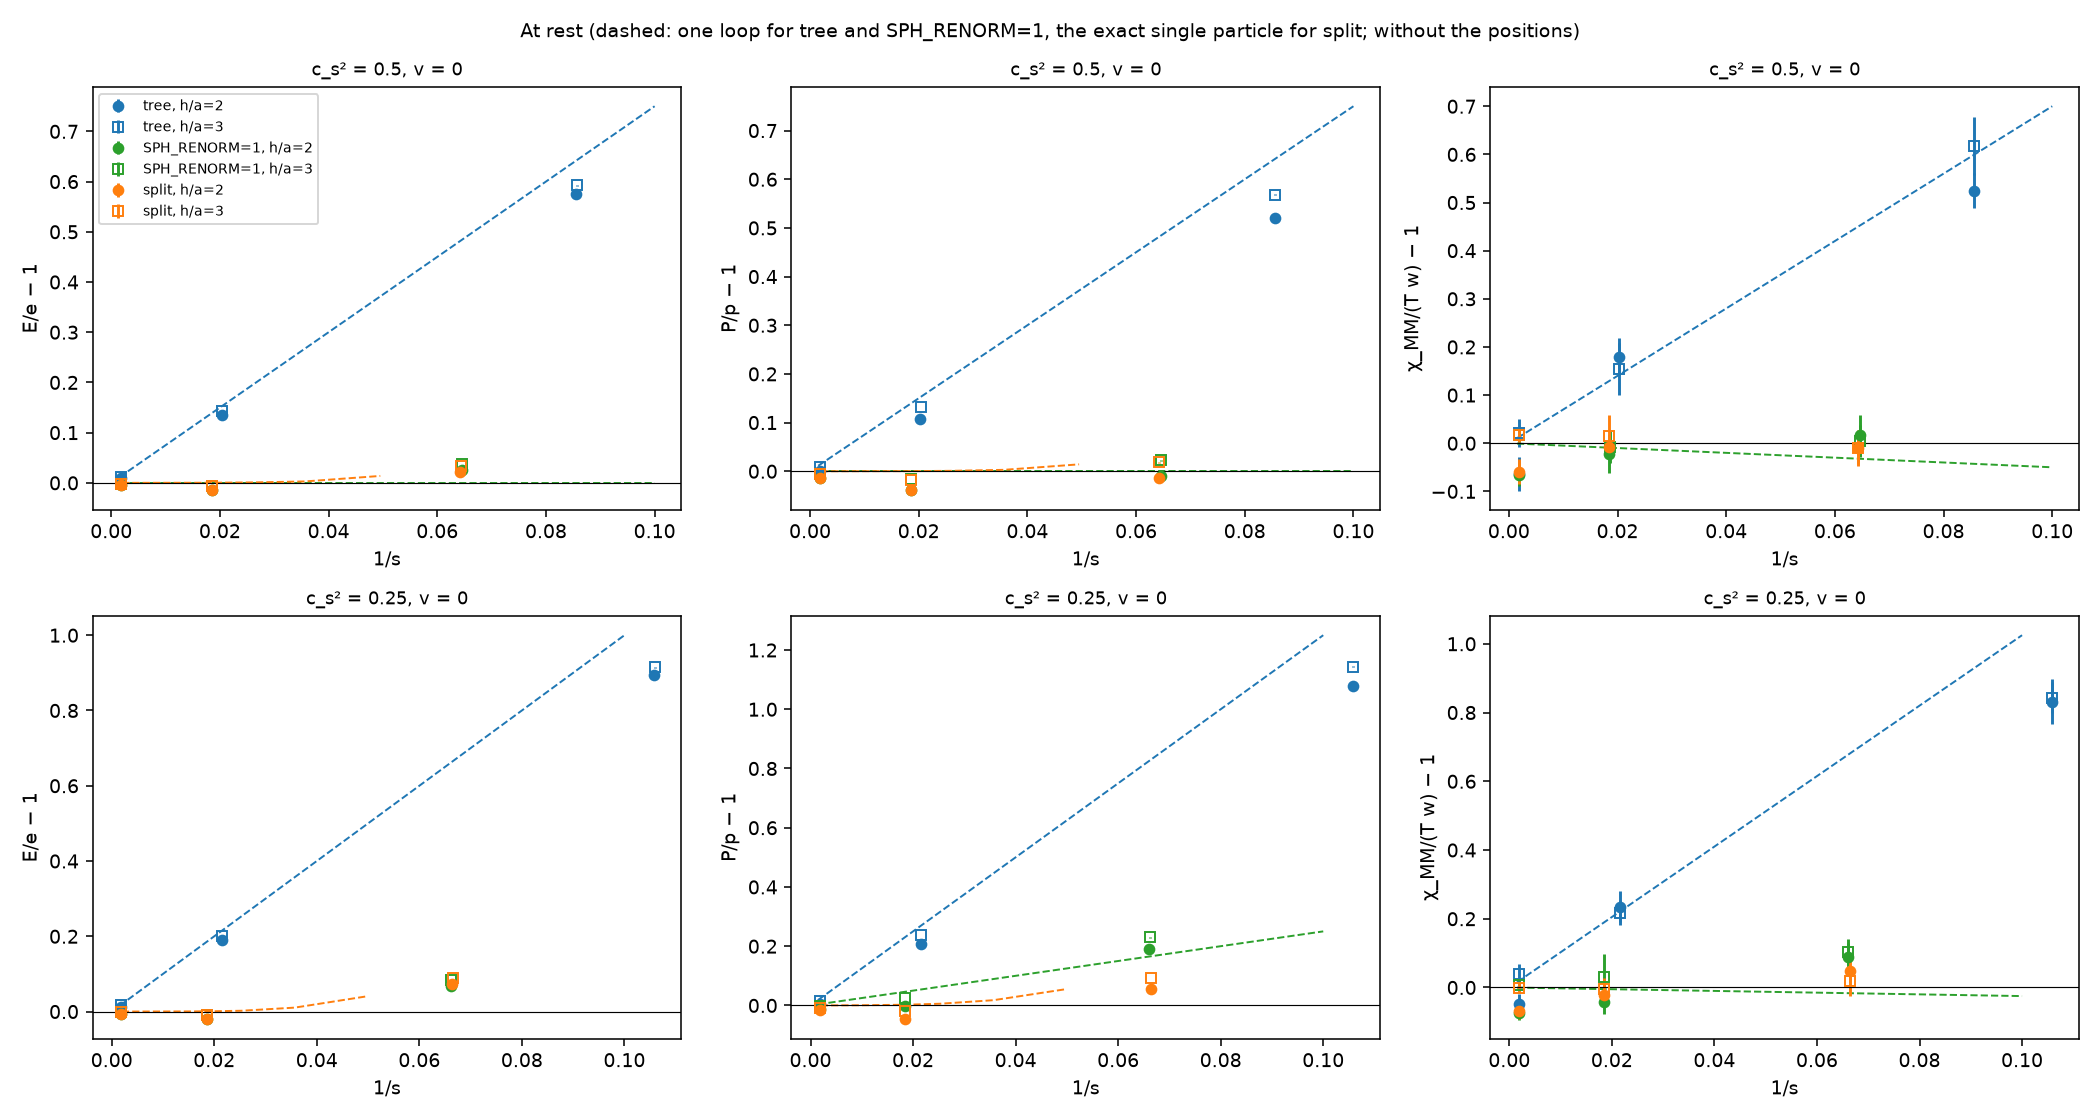
\includegraphics[width=\textwidth]{figs/split_EP.png}
\caption{Campaign \texttt{eos\_split} (\nolinkurl{step5_plan.tex}, Fig.~1).  At rest: $E/e-1$, $P/p-1$ and $\chi_{MM}/(Tw)-1$ against $1/s$ ($s$ the measured
entropy per particle), $c_s^2=1/2$ (top) and $1/4$ (bottom), $h/a=2$ (filled) and $3$ (open).  Blue: tree level; green: \texttt{SPH\_RENORM=1}, the
label part alone; orange: split.  Dashed: one loop for the tree level and \texttt{SPH\_RENORM=1} (at $c_s^2=1/4$ its pressure error $\mathcal N/\sigma$), the
exact single particle for split; without the positions.}
\label{fig:EP}
\end{figure}

\paragraph{Dynamics: campaign \texttt{hastings\_bath}} (\nolinkurl{split_dynamics.tex}; conformal, $d=2$, $\eta/s=0.2$, $s_a\in\{16,54\}$,
$v_0\in\{0,0.8\}$, the full dynamics with the stochastic step and its Hastings correction, against hybrid Monte Carlo of the same Hamiltonian, all at
the same bath $(T_{\rm rel},v_0)$).  (i) The dynamics with the split Hamiltonian samples its own equilibrium: its equal-time spectra over those of
its hybrid Monte Carlo are $1$ within $2$--$5\%$.  (ii) At $s_a=16$ the split equal-time spectra at the smallest $k$ match the susceptibilities of the
target equation of state, $C_{AA}(k,0)/\chi_{AA}=0.92$--$1.07$, where the tree level gives $1.2$--$1.4$ (\Fig{fig:eqt}); at $s_a=54$, split
$0.97$--$1.05$, tree $1.03$--$1.19$.  (When the tree level is started at the right energy instead of the right temperature it is low instead,
$0.85$ in the older campaign \texttt{hastings} at $c_s^2=\tfrac13$: the same $O(1/s_a)$ mismatch between temperature and energy.)  Advection is
unchanged, and the shear damping is similar for the two Hamiltonians.

\begin{figure}[h]
\centering
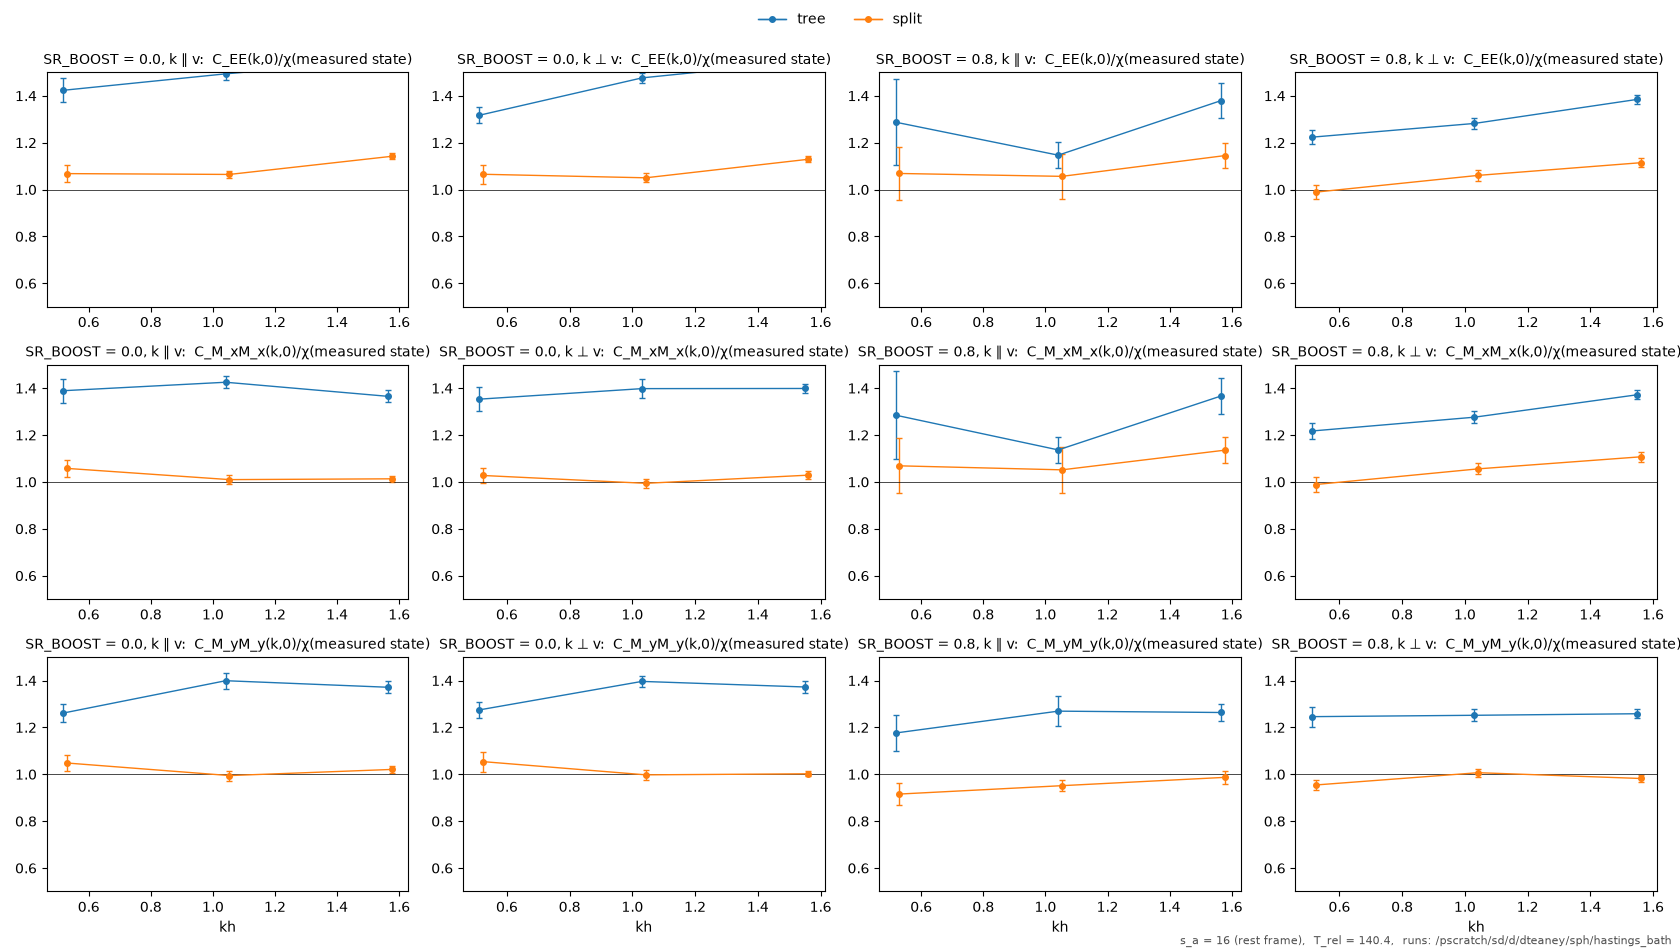
\includegraphics[width=\textwidth]{figs/boost_equaltime_SP16_bath.png}
\caption{Campaign \texttt{hastings\_bath} (commit \texttt{3262b00}; \nolinkurl{split_dynamics.tex}); run sets \texttt{hs16\_tr\_v<v>}, \texttt{hs16\_sp\_v<v>},
$s_a=16$, $v_0=0,0.8$.  $C_{AA}(k,0)/\chi_{AA}$ for $A=E,M_x,M_y$, $\bm k$ along and across the flow, $\chi$ of the target equation of state
($c_s^2=1/2$) at the bath; tree (blue), split (orange).}
\label{fig:eqt}
\end{figure}

%=============================================================================
\section{Open points}
\label{sec:open}

\paragraph{The default.}  \nolinkurl{split_dynamics.tex} states the intention to make \texttt{SPH\_RENORM=split} the default once its questions are
answered, and they are; but in the code at this commit the setting still defaults to off (\nolinkurl{src/stochastic.jl}, \texttt{setting("SPH\_RENORM",
false)}), i.e.\ the tree level.  This note calls split the chosen scheme; the owner has decided to make it the default (with \texttt{legendre} the alternative and
\texttt{SPH\_RENORM=0} the tree level), to be done with the merge of branch \texttt{split}.

\paragraph{Two older statements superseded.}  (i) \nolinkurl{renormalization_sph.tex} (abstract) says that no Hamiltonian makes the pressure at fixed
temperature independent of the density of particles, and proposes instead to tune the bare equation of state along curves of fixed $\mu/T$; its own
section ``Neutral labels'' and \nolinkurl{partition_v2.tex} construct exactly such a Hamiltonian ($\klab=0$), which is what both schemes implement.
(ii) \nolinkurl{partition_v2.tex}, ``The counterterm as shifts of the entropy and the momentum'', puts the sound term into a momentum shift
$\Delta\bm m_a$; the split scheme puts it into $H$ as the energy $E^{\rm dyn}$ at fixed $(u,\bm m)$, and the Legendre scheme shifts the momentum through
the transform.  These are schemes in the sense of \Sect{sec:common}, equal at one loop; the momentum-shift form was not implemented.

\paragraph{The term $\partial\Delta s^{\rm dyn}/\partial u$.}  \nolinkurl{partition.tex} (Step 5 and ``Step 5 for any $c_s^2$'') includes it in $E^{\rm dyn}$ as
$-\ln J^{\rm dyn}$; \nolinkurl{step5_plan.tex} (``Results'', A) drops it, and the code follows the latter.  The single-particle table of
\Sect{sec:compare} is from before the decision.

\paragraph{The damping at small bare viscosity.}  The shear and sound modes in \texttt{hastings\_bath} ($c_s^2=1/2$, $\eta/s=0.2$) decay 3--6 times
faster than hydrodynamics for the tree level and split alike, so this is not a property of the renormalization: it is the fluctuation
correction to the viscosity, large when the bare $\nu_0=(\eta/s)/T_{\rm rel}$ is small (campaigns \texttt{damping\_scan} and \texttt{cs13},
\nolinkurl{split_dynamics.tex}).  The point at $s_a=16$, $v_0=0.8$ along the flow ($11\pm3$ times hydrodynamics, short fit window) is the
noisiest instance of it.  Whether the $3$--$5\%$ of the weight within a few units of the label boundary at $s_a=16$ slows the votes or the
heat bath is open (\nolinkurl{step5_plan.tex}, ``Later'').

\end{document}
